\section{Evaluation}
\begin{frame}{Gesture Recognition}{Setup}
  \begin{itemize}
    \item Measure recognition time for $5, 10, \ldots, 100$ gesture traces
    \begin{itemize}
      \item Equal to $1, 2, \ldots, 20$ unique gestures, trained 5 times each
      \item Average of 60 measurements per number of gesture traces
    \end{itemize}
    \item Generate random gesture trace inputs
    \item Requirement: Faster than \SI{200}{\milli\second}
  \end{itemize}
\end{frame}

\begin{frame}{Gesture Recognition}{Performance}
  \vfill\centering
    \begin{tikzpicture}
    \begin{axis}[
    %      ybar,
    %      bar width=2pt,
    xlabel = Number of unique gestures,
    ylabel = Average time in ms,
    xtick=data,
    width=\textwidth,
    height = 6cm,
    yticklabel style={align=right,inner sep=0pt,xshift=-0.3em},
    enlargelimits = false,
    ymax = 150,
    grid=major,
    try min ticks=10]]
    \addplot table[x=gestureNo, y=time] {../data/three-dollar-test-results/results/10xrecognize/average.csv};   
    \end{axis}
    \end{tikzpicture}
\end{frame}

%Thalley: Usikker på om vi vil have memory med
%\begin{frame}{Gesture Recognition}{Memory}
%  \centering\vfill
%  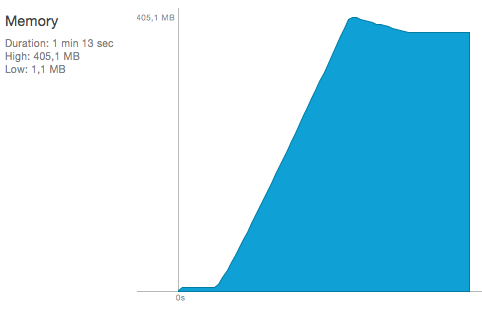
\includegraphics[width=0.9\textwidth]{../images/three-dollar-memory-use}
%\end{frame}

\begin{frame}{Gesture Recognition}{Correctness}
  \begin{itemize}
    \item Requirement: At least \perc{80}
    
    \item The authors report a correctness rate of \perc{80}
    \begin{itemize}
      \item Based on a study of 12 people
      \item Best score: \perc{98}
      \item Worst score: \perc{58}
    \end{itemize}
  \end{itemize}
\end{frame}

\begin{frame}{Precision of Indoor Positioning}{Setup}
  Tested in 4 settings:
  
  \begin{center}
    \scalebox{0.8}{
      \begin{tabular}{l| c c c c}
        Name   & Size in meters     & \# of Beacons   & \# of Tests & \# of WiFi Access Points \\ \hline
        Room 1 & $5 \times 5$       & \num{4}         & \num{8}     & \num{19}                 \\
        Room 2 & $8 \times 8$       & \num{4}         & \num{7}     & \num{19}                 \\
        Room 3 & $17.9 \times 17.9$ & \num{4}         & \num{3}     & \num{3}                  \\
        Room 4 & $4.90 \times 9.95$  & \num{4}/\num{8} & \num{33}    & \num{20}
      \end{tabular}
    }
  \end{center}
  
  \begin{center}
    \scalebox{0.7}{
      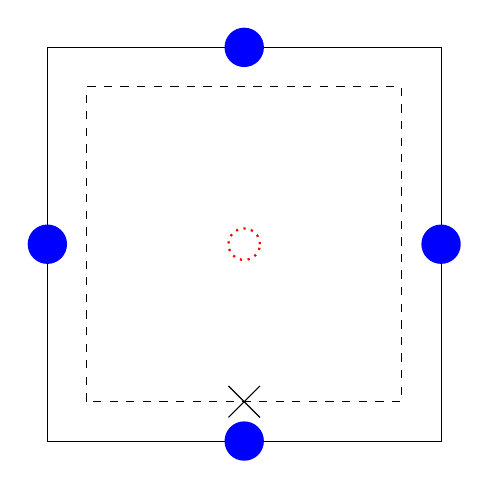
\begin{tikzpicture}

\draw (0,0) rectangle (5,5); % Outline of room

\draw[red,thick,dotted] (2.5,2.5) circle (0.2); % Phone location

\fill[blue!100!] (2.5, 0) circle (0.25); % Beacon location - Bottom
\fill[blue!100!] (5, 2.5) circle (0.25); % Beacon location - Right
\fill[blue!100!] (2.5, 5) circle (0.25); % Beacon location - Top
\fill[blue!100!] (0, 2.5) circle (0.25); % Beacon location - Left

% Walking path
\draw[dashed] (0.5,0.5) rectangle (4.5,4.5);

% Start / stop point of walking path
\draw (2.3,0.7) -- (2.7,0.3);
\draw (2.3,0.3) -- (2.7,0.7);

\end{tikzpicture}
    }
  \end{center}
\end{frame}

\begin{frame}{Precision of Indoor Positioning}{Auditorium Setup}
  \centering\vfill
  \includegraphics[width=\textwidth]{../drawings/audtest}
\end{frame}

\begin{frame}{Precision of Indoor Positioning}{Heatmap and Distance Graph (Room 4)}
	\centering\vfill
	  \begin{minipage}[b]{0.49\textwidth}
	  	\centering
	  	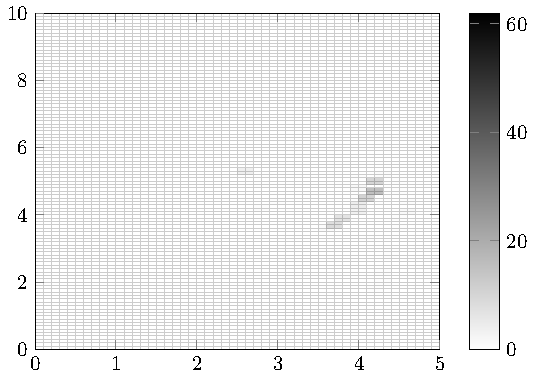
\includegraphics[width=\textwidth, height=4.5cm]{../data/estimote-test-results/heatmaps/pdf/36}
			\vspace{0.35cm}
%	  	\caption{Room 4, \SI{1}{\minute}, \num{4} beacons, centered}
%	  	\label{fig:room4:1:4:c}
	  \end{minipage}\hfill
	  \begin{minipage}[b]{0.49\textwidth}
	  	\centering      
	  	\begin{tikzpicture}
	  	\begin{axis}[
	  	height=\textwidth,
	  	width=\textwidth,
	  	ylabel = Distance in meters,
	  	xlabel = Measurements over time,
	  	enlargelimits=false,
	  	ymax=4,
	  	ymin=0,
	  	grid=major,
	  	max space between ticks=20pt,
%	  	xtick = {0, 50, 100, 150, 200, 250, 300}
	  	]
	  	\addplot table [x expr=\coordindex, y index=0] {../data/estimote-test-results/mean-error/36-1911-1027-490x995-1min.csv};
	  	\end{axis}
	  	\end{tikzpicture}
	  \end{minipage}
\end{frame}

\begin{frame}{Precision of Indoor Positioning}{Stationary Results}
  \centering
  \begin{tabular}{l|l c c c}
  	Room   & Position   & \# of beacons & \# of tests & Mean error        \\ \hline
  	Room 1 & Centered   & \num{4}       & 5           & \SI{1.78}{\meter} \\
  	Room 2 & Centered   & \num{4}       & 4           & \SI{2.96}{\meter} \\
  	Room 3 & Centered   & \num{4}       & 3           & \SI{7.31}{\meter} \\
  	Room 4 & Centered   & \num{4}       & 3           & \SI{1.94}{\meter} \\
  	Room 4 & At $(2,8)$ & \num{4}       & 3           & \SI{1.22}{\meter} \\
  	Room 4 & Centered   & \num{8}       & 3           & \SI{3.02}{\meter} \\ \hline
  	Total  &            &               & 31          & \SI{2.92}{\meter}
  \end{tabular}
\end{frame}

\begin{frame}{Impact of Simulated Accuracy}{Setup}
  \begin{itemize}
    \item Given the result of the precision test, how does the system work?
    \item Simulate a inaccurate position on the circle with radius \SI{2.92}{\meter}
  \end{itemize}
  \begin{center}
    \scalebox{0.8}{
    	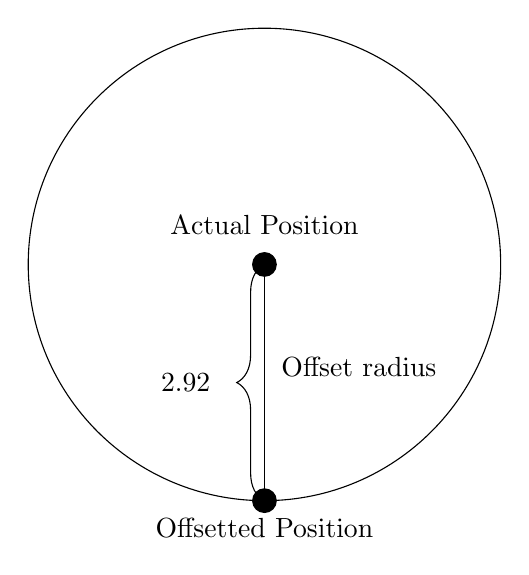
\begin{tikzpicture}
    	\draw[fill] (5, 5) circle (0.15); % Inner cirlce
    	\draw (5, 5) circle (3); % Outer cirlce
    	\draw (5, 5) -- (5,2); % Radius
    	\draw[fill] (5, 2) circle (0.15);
    	
    	%Text
    	\node at (5,5.5) {Actual Position};
    	\node at (5,1.65) {Offsetted Position};
    	\node at (6.2, 3.7) {Offset radius};
    	
    	\draw [decorate,decoration={brace,amplitude=10pt,mirror}] (5,5) -- (5,2) node[midway, xshift=-1cm] {\SI{2.92}{\meter}};
    	\end{tikzpicture}
    	}
  \end{center}
\end{frame}

\begin{frame}{Impact of Simulated Accuracy}{Setup}
  \begin{itemize}
    \item 18 tests with different positions
    \item 6 devices in room of size $6.9 \times 5.37$ meters
    \begin{itemize}
      \item 3 test for each focused device
    \end{itemize}
    \item Requirement: At least \perc{80} accuracy
  \end{itemize}
\end{frame}

\begin{frame}{Impact of Simulated Accuracy}{Results}
  \centering\vfill
  \begin{tikzpicture}
  \begin{axis}[
    xlabel = Offset in meters,
    ylabel = Accuracy in percent,
    xtick=data,
    width=\textwidth,
    height = 6cm,
    yticklabel style={align=right,inner sep=0pt,xshift=-0.3em},
    enlargelimits = false,
    ymax = 100,
    ymin = 0,
    nodes near coords align={right},
    nodes near coords={\pgfmathprintnumber\pgfplotspointmeta\%},
    every node near coord/.append style={font=\footnotesize, inner sep=1pt, yshift=0.2cm},
    grid=major,
    try min ticks=10]
    \addplot table[x=offset, y=accuracy] {../data/system-correctness/results.csv};   
  \end{axis}
  \end{tikzpicture}
\end{frame}


